\documentclass[10pt, aspectratio=169]{beamer}

% --- Paquetes ----------------------------------------------------------------
\usepackage[utf8]{inputenc}
\usepackage[T1]{fontenc}
\usepackage[spanish]{babel}
\usepackage{graphicx}
\usepackage{booktabs}
\usepackage{listings}
\usepackage{multicol}
\usepackage[table]{xcolor} % UNA SOLA VEZ Y CON [table]
\usepackage{booktabs}
\usepackage{xltabular}
\usepackage{caption}
\usepackage{subcaption}
\usepackage{array}
\usepackage{multirow}
% --- Configuración de Colores (Estilo UVa) ------------------------------------
\definecolor{azulUVa}{RGB}{0, 51, 153}
\definecolor{rojoUVa}{RGB}{193, 0, 60}
\setbeamercolor{palette primary}{bg=azulUVa,fg=white}
\setbeamercolor{palette secondary}{bg=rojoUVa,fg=white}
\setbeamercolor{palette tertiary}{bg=black,fg=white}
\setbeamercolor{structure}{fg=azulUVa}

\usetheme{Madrid}

% --- Configuración de Código --------------------------------------------------
\lstset{
	language=Java,
	basicstyle=\ttfamily\tiny,
	keywordstyle=\color{blue},
	commentstyle=\color{green!60!black},
	stringstyle=\color{rojoUVa},
	breaklines=true,
	tabsize=2,
	showstringspaces=false
}

% --- Datos de la Portada -----------------------------------------------------
\title[Card Partner]{Card Partner: All-in-One TCG Platform}
\subtitle{Servicios y Sistemas Web}
\author[Grupo 33]{Álvaro,Edgar,Marcos y Sergio}
\institute[UVa]{Universidad de Valladolid}
\date{Curso 25-26}

% -----------------------------------------------------------------------------
\begin{document}
	
	% --- Slide 1: Portada ---
	\begin{frame}
		\titlepage
	\end{frame}
	
	% --- Slide 2: Índice ---
	\begin{frame}{¿Qué vamos a ver hoy?}
		\begin{columns}[t]
			\begin{column}{0.5\textwidth}
				\tableofcontents[sections={1-3}]
			\end{column}
			\begin{column}{0.5\textwidth}
				\tableofcontents[sections={4-6}]
			\end{column}
		\end{columns}
	\end{frame}
	
	\section{Presentación del grupo 33}
	\begin{frame}{¿Quiénes somos los creadores de \textit{Card Partner}?}
		\begin{table}
			\centering
			\scriptsize % Reducimos la fuente para que el texto largo no sature la slide
			\renewcommand{\arraystretch}{1.2}
			% Ajustamos columnas proporcionalmente al ancho de la diapositiva (Suma 0.90)
			\begin{tabular}{|>{\raggedright\arraybackslash}p{0.25\textwidth}|>{\centering\arraybackslash}p{0.10\textwidth}|>{\raggedright\arraybackslash}p{0.55\textwidth}|}
				\hline
				\textbf{Nombre} & \textbf{\%} & \textbf{Responsabilidad principal} \\
				\hline
				\hline
				\multicolumn{3}{|c|}{\textbf{Equipo Frontend}} \\
				\hline
				Marcos  & 25\% & Vistas de cartas, apartado social, navegabilidad general, revisión visual y maquetación. \\
				\hline
				Sergio  & 25\% & Vistas de mazos, login, registro, página principal, constructor de mazos e integración visual. \\
				\hline
				\hline
				\multicolumn{3}{|c|}{\textbf{Equipo Backend y Gestión de Datos}} \\
				\hline
				Álvaro  & 25\% & Esquema BBDD, colaboración modelo E-R, población de datos, \textit{scripts} MariaDB en local y redacción técnica. \\
				\hline
				Edgar  & 25\% & creación modelo E-R, esquemas BBDD, clases del modelo, DAOs y DTOs. \\
				\hline
			\end{tabular}
		\end{table}
	\end{frame}
	
	\section{El Concepto \textit{Card Partner}}
	\begin{frame}{Contexto y Problema}
		
		\begin{itemize}
			\item \textbf{Crecimiento de los TCG:} este \textit{hobby} ha ganado mucha popularidad en los últimos años.
			\item \textbf{Información Dispersa:} los jugadores deben desplazarse entre diferentes webs para conseguir la información necesaria
			\item \textbf{Barrera de Entrada:} los principiantes se sienten abrumados por un mundo tan complejo.
		\end{itemize}
		\vspace{0.3cm}
		\begin{block}{Nuestra Propuesta}
			Una aplicación web \textbf{All-in-One} que centraliza catálogo, mercado, construcción de mazos y comunidad en una experiencia fluida.
		\end{block}
	\end{frame}
	
	\section{Diferencia con las aplicaciones actuales}
	\begin{frame}{¿Por qué Card Partner es diferente?}
		A diferencia de sitios como \textit{Card Market} o \textit{Limitless TCG}, nosotros aportamos:
		\vspace{0.3cm}
		\begin{description}
			\item[Enfoque Social:] buscamos generar una comunidad de jugadores en nuestra aplicación.
			\item[Gestión de Colección:] \textit{wishlist} integrada para facilitar la gestión del catálofo de cartas.
			\item[Inteligencia Contextual:] traducción de jerga técnica asistida por IA.
			\item[Visualización Dinámica:] constructor de mazos con filtros inteligentes basados en el líder. seleccionado.
		\end{description}
	\end{frame}
	
\section{Arquitectura del Sistema}
\begin{frame}{Tecnologías empleadas y BBDD}
	\begin{columns} % <-- AQUÍ PLURAL
		
		\begin{column}{0.6\textwidth} % <-- ABRES COLUMNA 1
			\textbf{Backend \& Frontend:}
			\begin{itemize}
				\item JSP y Servlets (Arquitectura MVC).
				\item DAOs para abstracción de persistencia.
				\item Base de Datos MariaDB (Relacional).
			\end{itemize}
			\textbf{Pilares de Información:}
			\begin{itemize}
				\item Usuarios (Roles: Jugador, Editor, Admin).
				\item Catálogo Técnico (Cartas, Atributos, Precios).
				\item Interacción (Comentarios, Valoraciones, Wishlist).
			\end{itemize}
		\end{column} % <-- CIERRAS COLUMNA 1
		
		\begin{column}{0.4\textwidth} % <-- ABRES COLUMNA 2
			\begin{figure}
				\centering
				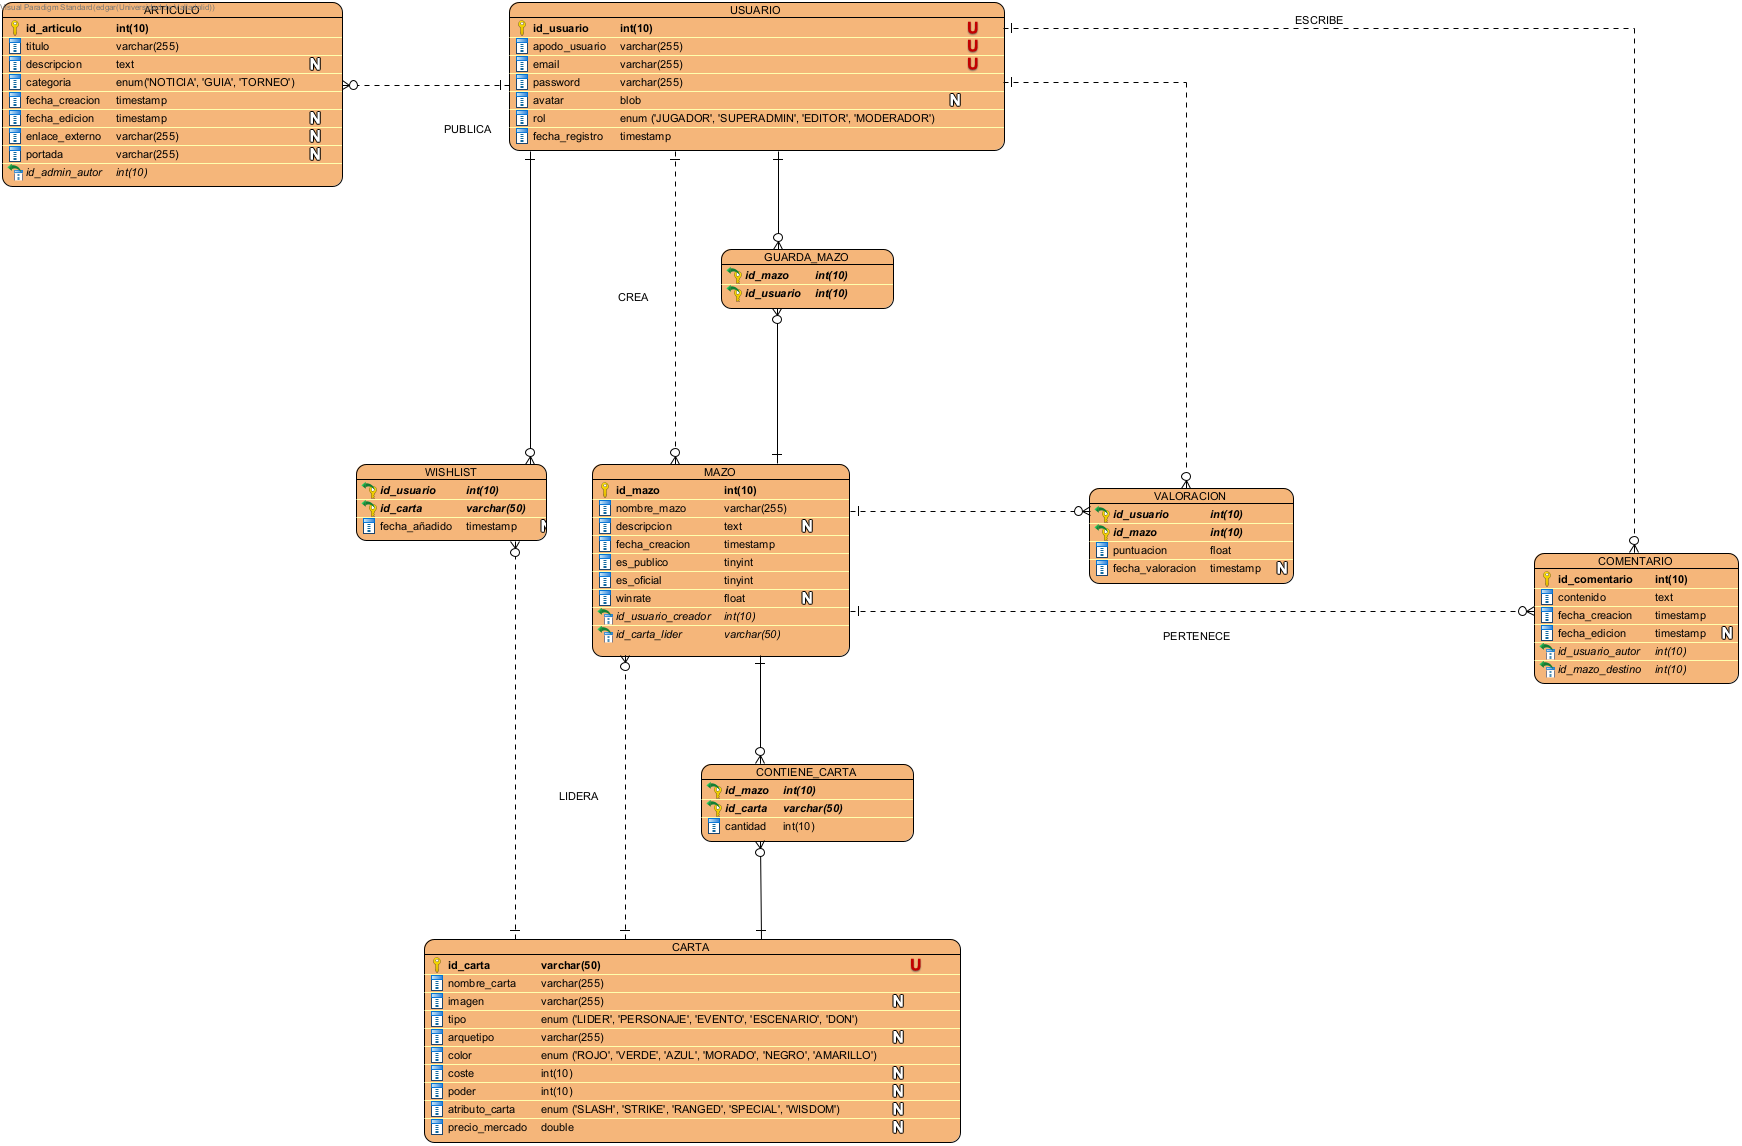
\includegraphics[width=\textwidth]{Recursos/CardPartner_DBv2.png}
				\caption{Esquema Relacional}
			\end{figure}
		\end{column} % <-- CIERRAS COLUMNA 2
		
	\end{columns} % <-- AQUÍ PLURAL
\end{frame}
			
\begin{frame}{Integración de APIs: OPTCG API}
	\begin{columns}[c] % Alineación centrada verticalmente
		% --- Columna de Texto (55% del ancho) ---
		\begin{column}{0.55\textwidth}
			\textbf{Reto:} Sincronizar +2000 cartas manualmente es inviable.
			
			\begin{itemize}
				\item \scriptsize \textbf{Consumo REST:} Uso de \textbf{GSON} para el parseo de JSONs masivos de forma eficiente.
				\item \scriptsize \textbf{Artes Alternativos:} Algoritmo con \texttt{HashMap} para evitar colisiones de ID asignando sufijos (\texttt{\_p1}, \texttt{\_p2}).
				\item \scriptsize \textbf{Robustez:} Sanitización de datos y validación de formatos en la capa de persistencia.
			\end{itemize}
			
			\begin{exampleblock}{Resultado}
				\small Base de datos siempre actualizada con los lanzamientos de Bandai de forma autónoma.
			\end{exampleblock}
		\end{column}
		
		% --- Columna de Imágenes (40% del ancho) ---
		\begin{column}{0.40\textwidth}
			\centering
			\begin{figure}
				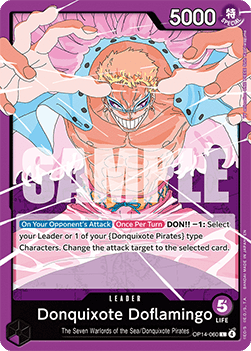
\includegraphics[width=0.45\textwidth]{Recursos/dfV1.png}
				\vspace{0.3cm} % Espacio entre imágenes
				
\includegraphics[width=0.45\textwidth]{Recursos/dfV2.png}
				\caption{\tiny Evolución de los datos}
			\end{figure}
		\end{column} % <-- Aquí estaba el fallo (antes ponía </column>)
	\end{columns}
\end{frame}
			
		\begin{frame}[fragile]{Traducción contextual (Gemini/Groq)}
			\textbf{Reto:} Permitir que usuarios con distintos idiomas puedan emplear nuestra \textit{app}
			\begin{itemize}
				\item \textbf{Llama-3 via Groq:} integración mediante HTTP Post.
				\item \textbf{Prompts Dinámicos:} la AI recibe instrucciones distintas según si traduce un mazo (técnico) o un comentario (natural).
				\item \textbf{Tolerancia a Fallos:} si la API no responde, el sistema muestra el texto original sin romper la interfaz.
			\end{itemize}
			\vspace{0.2cm}
			\begin{lstlisting}
				String instruccion = switch (tipo) {
					case "MAZO" -> "Translate using TCG jargon (Ramp, OTK). ONLY output text: ";
					...
				};
			\end{lstlisting}
		\end{frame}
			
			\section{Funcionalidades Estrella}
			\begin{frame}{Puntos fuertes de la aplicación}
				\begin{itemize}
					\item \textbf{Constructor de Mazos:} ventanas modales y filtros automáticos por color/arquetipo del líder para facilitar la creación de \textit{decks}.
					\item \textbf{InteracciónSocial:} posibilidad de generar una comunidad mediante las propuestas de interacción entre usuarios que hemos desarrollado.
					\item \textbf{Precios realistas}: permitimos a los usuarios consultar un precio de mercado realista de las cartas.
					\item \textbf{TCG Hub:} estructura preparada para escalar a otros juegos (Magic, Pokémon) con una simple adaptación al formato
				\end{itemize}
			\end{frame}
			
			\section{Conclusión}
			\begin{frame}{Trabajo Realizado y Futuro}
				\begin{itemize}
					\item \textbf{Logro:} hemos transformado un concepto estático en una herramienta funcional capaz de gestionar miles de registros.
					\item \textbf{Tecnología:} ha combinación de DAOs sólidos y APIs externas nos da una escalabilidad profesional.
					\item \textbf{Próximos Pasos:} implementación de los diferentes TCGs, posibilidad de hacer un apartado de \textit{marketplace} para poder intercambiar las cartas.
				\end{itemize}
			\end{frame}
			\section{Demo técnica}
			\begin{frame}{Vamos a ver \textit{Card Partner} en funcionamiento}
			\begin{figure}[H]
				\centering
				\includegraphics[width=0.8\textwidth]{Recursos/Kalgara.png}
			\end{figure}
			\end{frame}
			\begin{frame}{Despedida}
				\centering
				\Huge \textcolor{azulUVa}{\textbf{¡Muchas gracias!}}\\
				\vspace{0.5cm}
				\Large{¿Preguntas?}
		\end{frame}
		
	\end{document}